\documentclass[10pt,hyperref={colorlinks,linkcolor=black,citecolor=blue,urlcolor=blue!70},handout]{beamer}
\usepackage[mode=buildnew]{standalone}
\usepackage[utf8]{inputenc}
\usepackage[catalan]{babel}
\usepackage{tikz}
\usepackage{pgfplots}
\usepackage{graphicx}
\usepackage{animate}
\usepackage{stmaryrd}
\usepackage[absolute,overlay]{textpos}

%%% url symbol for references it is needed \usepackage{stmaryrd} %%%
\newcommand\enllas{\raise.5pt\hbox{$\boxempty\kern-4.85pt{}^{\nearrow}$}\kern-2pt}
%%%%%%%%%%%%%%%%%%%%%%%%%%%%%%%%%%%%%%%%%%%%%%%%%%%%%%%%%%%%%%%%%%%%

\newcommand\FrameText[1]{
  \begin{textblock*}{\paperwidth}(15pt,0.95\textheight)
    \tiny
    \raggedright #1\hspace{.5em}
  \end{textblock*}}

\usetheme{Copenhagen}
\usecolortheme{seahorse}

\pgfplotsset{compat=newest}

\DeclareMathOperator{\diss}{diss}
\DeclareMathOperator{\arccosh}{arccosh}

\definecolor{color1}{RGB}{255,158,1}
\definecolor{color2}{RGB}{255,74,1}
\definecolor{color3}{RGB}{220,0,0}
\definecolor{color4}{RGB}{180,0,0}
\definecolor{lessgreen}{RGB}{0,100,0}

\institute[UAB]{Taller de modelització\\
\vspace{5pt}Grau en Matemàtiques\\
\vspace{5pt}Universitat Autònoma de Barcelona}
\title[Mesures de dissonància]{Mesures de dissonància}
\author[Víctor, Oriol, Carlo]{Víctor Ballester\and Oriol Bosquet \and Carlo Sala}
\date{Març 2021}

\newtheorem{defin}[theorem]{Definició}

\begin{document}
\frame{\titlepage}
\begin{frame}{Enunciat i objectius}
  Podem resumir l'enunciat en 2 punts bàsics:\pause
  \begin{itemize}
    \item Proposar una fórmula concreta per a la mesura del grau de dissonància.\pause
    \item Comprovar que aquesta fórmula concorda amb les dades empíriques de la percepció de la dissonància.\pause
  \end{itemize}
  Ens marquem 2 objectius:\pause
  \begin{itemize}
    \item Donar una fórmula de creació pròpia al més acurada possible.\pause
    \item Comprovar mitjançant un test fet a un grup divers de persones com s'entén la dissonància (o consonància).
  \end{itemize}
\end{frame}
\begin{frame}{Definició de dissonància i consonància}
  El diccionari de l'Institut d'Estudis Catalans ens diu:\\\pause
  \textbf{Dissonància.} Qualitat de dos o més sons que formen una combinació inharmoniosa, poc agradable a l'orella.\\
  \textbf{Consonància.} Qualitat de dos sons que, produïts simultàniament, formen un interval d'un acord perfecte.\\\pause
  \vspace{0.4cm}
  Proposem nosaltres la nostra pròpia definició:\\\pause
  \textbf{Dissonància.} Qualitat de dos o més sons amb una relació de freqüències concreta, que sonen poc agradables a l'oïda humana.\\
  \textbf{Consonància.} Qualitat de dos o més sons amb una relació de freqüències concreta, que sonen agradables a l'oïda humana.\\\pause
  \vspace{0.2cm}
  A més distingirem dos tipus de sons:\\\pause
  \textbf{So pur.} Ona sinusoidal formada per una sola freqüència, amplitud i fase.\\
  \textbf{So complex.} Suma d'un nombre arbitrari de sons purs. Si les freqüències relatives a aquests sons purs són totes múltiples d'una freqüència fonamental, el so complex s'anomena \textit{harmònic} i els seus components, \textit{harmònics}.
\end{frame}
\begin{frame}{Un primer model simple}
  Considerem dos sons purs de mateixa amplitud $A$, freqüències $f_1$ i $f_2$ i angle de fase $\phi=0$. És a dir, dos sons de la forma: $$y_1(t)=A\sin(2\pi f_1t)\qquad y_2(t)=A\sin(2\pi f_2t)$$\pause
  Si fem la superposició dels dos sons obtenim: $$y(t)=y_1(t)+y_2(t)=2A\cos\left(2\pi\frac{f_1-f_2}{2}t\right)\sin\left(2\pi\frac{f_1+f_2}{2}t\right)$$
\end{frame}
\begin{frame}{}
  Si considerem $A=1$, $f_1=10\text{ Hz}$ i $f_2=11\text{ Hz}$:\par\pause
  \begin{figure}
    \centering
    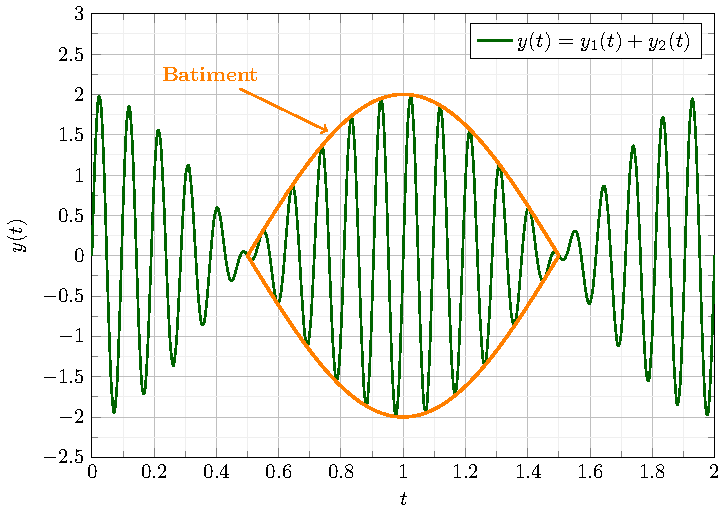
\includegraphics[width=8cm]{Imatges_beamer1/sin2.tex}
  \end{figure}
  Freqüència de batiment: $\frac{f_1-f_2}{2}\qquad$ Freqüència de propagació: $\frac{f_1+f_2}{2}$\par\pause
  Els batiments són el que ens provoca la dissonància.
\end{frame}
\begin{frame}{}
  Això es tradueix a:
  \begin{itemize}
    \item Si $|f_1-f_2|<10\text{ Hz}$: Interpretem un únic so i podem distingir els batiments.\pause
    \item Si $10\text{ Hz}<|f_1-f_2|<60\text{ Hz}$: Els sons estan massa separats per ser interpretats com un de sol, però massa junts per distingir-se amb claredat. Es produeix \textbf{dissonància}.\pause
    \item Si $|f_1-f_2|>60\text{ Hz}$: Podem distingir els dos sons. Es produeix \textbf{consonància}.
  \end{itemize}
  \FrameText{George N. Gibson, Ph.D. \textit{The Music of Physics}.\href{https://www.phys.uconn.edu/~gibson/Notes/Section5_5/Sec5_5.htm}{\enllas}.}
\end{frame}
\begin{frame}{Analogia de la interpretació de dos sons purs}
  Veiem una analogia amb l'animació següent reproduïda a diferents fotogrames per segon.\par
  \begin{center}
    \animategraphics[controls,width=7cm,loop]{60}{Imatges_beamer1/gif/fps-}{0}{89}
  \end{center}
  \FrameText{\textit{Compare frames per second}.\href{https://frames-per-second.appspot.com/}{\enllas}.}
\end{frame}
\begin{frame}
  Per calcular una fórmula, hem usat enginyeria inversa:\par
  \begin{center}
    Estimar els valor que voldríem $\longrightarrow$ Crear una funció adequada
  \end{center}\pause
  Fixada una freqüència $f_1$, si fem variar $r:=\frac{f_2}{f_1}$:\pause
  \begin{figure}
    \centering
    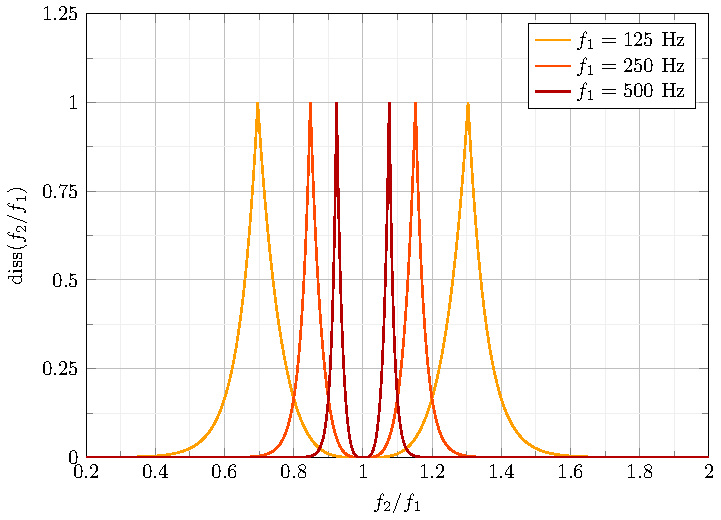
\includegraphics[width=6cm]{Imatges_beamer1/formula1.tex}
  \end{figure}\pause
  \scriptsize{$$\diss(r)=
      \left\{\begin{array}{lll}
        e^{\beta f_1(r-1+\gamma_{f_1})}                                 & \text{si} & 0<r<1-\gamma_{f_1}                          \\
        \cosh\left[\frac{\arccosh(2)}{(\gamma_{f_1})^2}(r-1)^2\right]-1 & \text{si} & 1-\gamma_{f_1}<r<1+\gamma_{f_1}\vspace{5pt} \\
        e^{-\beta f_1(r-1-\gamma_{f_1})}                                & \text{si} & 1+\gamma_{f_1}<r
      \end{array}\right.$$ on $\beta$ és una constant i $\gamma_{f_1}\propto\frac{1}{f_1}$.}
\end{frame}
\begin{frame}{Exemples}
  Escoltem ara els exemples següents partint de $f_1=220\text{ Hz}$.
  \begin{itemize}
    \item\only<1| handout:1>{$f_2=225\text{ Hz}$: \beamerbutton{Play}
      \begin{figure}
        \centering
        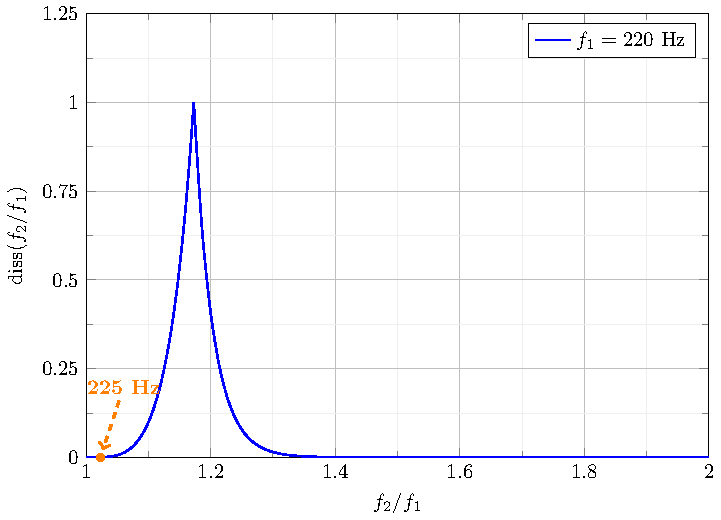
\includegraphics[width=8cm]{Imatges_beamer1/formula1_exemple1.tex}
      \end{figure}}
    \only<2| handout:2>{$f_2=258\text{ Hz}$: \beamerbutton{Play}
      \begin{figure}
        \centering
        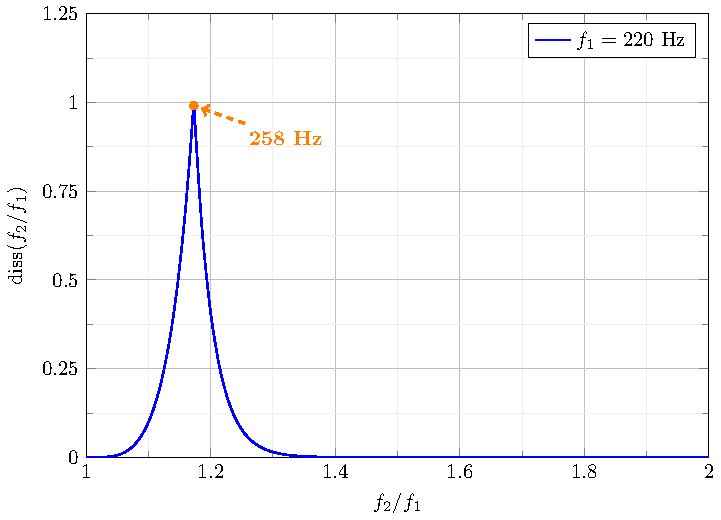
\includegraphics[width=8cm]{Imatges_beamer1/formula1_exemple2.tex}
      \end{figure}}
    \only<3| handout:3>{$f_2=320\text{ Hz}$: \beamerbutton{Play}
      \begin{figure}
        \centering
        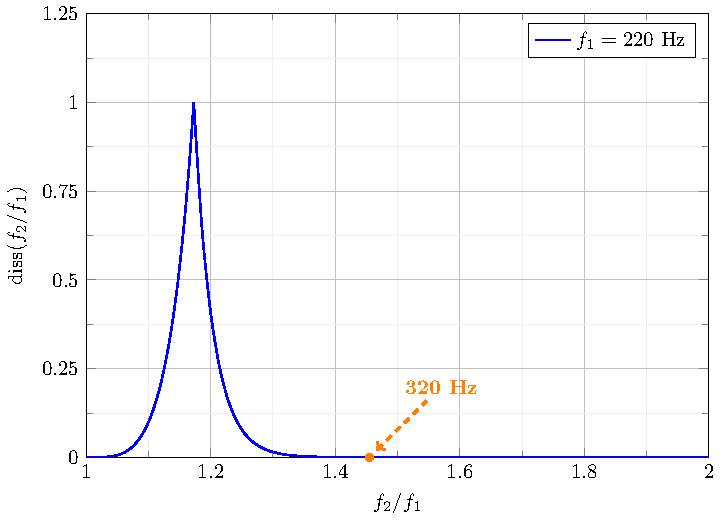
\includegraphics[width=8cm]{Imatges_beamer1/formula1_exemple3.tex}
      \end{figure}}
  \end{itemize}
\end{frame}
\begin{frame}{Possibles extensions}
  Tenim pensats dos refinaments:
  \begin{enumerate}
    \item Estudiar com l'oïda humana interpreta els fenòmens auditius i si pot interferir substancialment en la fórmula proposada.\pause
    \item Estudiar sons complexos, com el d'un instrument real.\par\pause
          Hi ha noves variables que entren en joc:
          \begin{itemize}
            \item Els harmònics\pause
            \item L'amplitud de les ones\pause
          \end{itemize}
          \vspace{0.5cm}
          Idea de la construcció de la fórmula final:
  \end{enumerate}
  $$\boxed{\parbox{3.5em}{\centering So complex}}\xrightarrow{\parbox{4.8em}{\centering\scriptsize Transformada de Fourier}}\boxed{\parbox{6em}{\centering Freqüències i amplituds dels harmònics}}\xrightarrow{\parbox{4.8em}{\centering\scriptsize Fórmula per a sons simples}}\boxed{\parbox{4.5em}{\centering Suma ponderada entre els harmònics}}$$
\end{frame}
\begin{frame}{Experiment final}
  Un cop trobada una fórmula per a la dissonància de sons complexos, hem pensat de fer un petit test per corroborar el nostre model.\par\pause El test tindrà l'aspecte següent:
  \begin{itemize}
    \item Anirà dirigit a un públic general (incloent persones amb oïda entrenada i no entrenada).\pause
    \item Els preguntarem com de dissonant sonen diversos sons complexos.\pause
    \item Compararem el nostre model amb els fets empírics.
  \end{itemize}
\end{frame}
\end{document}

